% --------------------------------------
% Chapter 6 Solutions
% --------------------------------------

\subsection{6.1 $\bigstar$}
Suppose $x>0$. Then $|x|=x$, and so
$$\theta(x)=\frac{x+x}{2x}=1$$
If $x<0$, then $|x|=-x$, and so
$$\theta(x)=\frac{-x+x}{2x}=0$$


\subsection{6.2 $\bigstar \bigstar \bigstar$}
The technique to prove this is almost identical to that in problem [6.4], which we have worked out in detail.


\subsection{6.3 $\bigstar$}
It seems that the relevant rules are in the beginning of section 6.5, rather than at the end. \\ \\ To show this, we simply differentiate, then set to 0. Then differentiate again and again set to zero, etc. In this way we get each of the coefficients $a_n$. So iff $f(x)=a_0+a_1 x+a_2 x^2+\ldots$ then obviously $f(0)=a_0$. Differentiating once, 
$$\frac{\dd f(x)}{\dd x}=a_1+2a_2 x+3a_3 x^2+\ldots$$
So then $f'(0)=a_1$. To get the $n^{th}$ term, we evidently have to differentiate $n$ times and set to zero.
\begin{align*}\frac{\dd^n f(0)}{\dd x^n}&=n(n-1)(n-2)\ldots 1\cdot a_n+(n+1)\cdot n \cdot(n-1)\ldots 1 a_{n+1}0+ \ldots\\
&=n!a_n
\end{align*}
and so $$a_n=\frac{f^{(n)}(0)}{n!}$$.


\subsection{6.4 $\bigstar \bigstar \bigstar$}
To show that the function 
$$f(x)=e^{-\frac{1}{x^2}}$$
is $C^{\infty}$ we need to show that each of its derivatives is continuous. Iff we differentiate once, we get
$$\frac{\dd f(x)}{\dd x}=\frac{2 e^{-\frac{1}{x^2}}}{x^3}$$
If we differentiate more often, we will see a pattern: each derivative is a sum of terms of the form $A x^{-n} e^{-\frac{1}{x^2}}$ where $A$ is some constant. Indeed
$$\frac{\dd }{\dd x}\left(\frac{e^{-\frac{1}{x^2}}}{x^n}\right)=\frac{2 e^{-\frac{1}{x^2}}}{x^{n+3}}-\frac{n e^{-\frac{1}{x^2}}}{x^{n+1}}$$
So if one derivative is a sum of terms of the form $A x^{-n} e^{-\frac{1}{x^2}}$, then all subsequent derivatives will also be of this form, which is what we claimed. \\ \\ Now iff the term $A x^{-n} e^{-\frac{1}{x^2}}$ is continuous, we note that that finite sums of these terms are also continuous. Let us first show continuouity\footnote{We say a function $f(x)$ is continuous at $x=0$ iff $\lim_{x\to 0} f(x)$ is the same whether the limit goes from above or below.} $x=0$. \\ \\ We see that as $x\to 0^\pm$, $e^{-1/x^2}\to 0$ and $x^{-n}\to \pm \infty$. So does $e^{-1/x^2}$ tend to 0 faster than $x^{-n}$ tends to $\infty$? The answer is yes. To see this, consider the power-series\footnote{We could also use \emph{L'Hospitals Rule} here.} obtained by expanding the exponent: 
\begin{align*}
e^{1/x^2}&=1+\frac{1}{x^2}+\frac{1}{2!\cdot x^4 }+\ldots \frac{1}{(n+1)!\cdot x^{2n+1}}+\ldots  > \frac{1}{(2n+1)!\cdot x^{2n+1}}\\
\implies  \ \ \ \ \ e^{-\frac{1}{x^2}}&< (2n+1)!\cdot x^{2n+1}\\
\implies \ \ \ \ \ \lim_{x\to 0}\frac{e^{-\frac{1}{x^2}}}{x^n}&<\lim_{x\to 0} \frac{(2n+1)!x^{2n+1}}{x^n}=(2n+1)!\lim_{x\to 0} x^{n+1}=0
\end{align*}
The argument above applies regardless of whether the limit is from above or below, and hence every derivative is continuous at $x=0$. It is easy to see that the function is continuous everywhere else, as we know in general that if $I$ and $J$ are intervals, $f:I\to\mathbb{R}$ is continuous at $x\in I$ ($f(x)\in J$) and $g: J\to \mathbb{R}$ is continuous at $f(x)$, then the composition $g\circ f$ is also continuous at $x$. In our case, $f(x)=e^x$ and $g(x)=-x^{-2}$ which are both obviously continuous at $x\neq 0$, and hence the composition of them is also continuous on this domain. Muliplying this with $x^{-n}$ will again yield a continuous function (in the defined domain), as multiplying continuous functions preserves continuouity.  And so we have that $k(x)=A x^{-n} e^{-\frac{1}{x^2}}$ is continous for all $\mathbb{R}$, and hence all the derivatives of $f(x)=e^{-\frac{1}{x^2}}$ are continuous, and hence our function is $C^{\infty}$ smooth. 
\\ \\ Now we need to show that $f(x)=e^{-\frac{1}{x^2}}$ is not analytic at $x=0$. This is easy, as suppose $f(x)$ can be expressed by a power series about $x=0$. Then 
$$f(x)=f(0)+\frac{f'(0)}{1!}x+\frac{f''(0)}{2!}x^2+\frac{f'''(0)}{3!}x+\ldots$$
But we have just shown that each derivative vanishes at $x=0$. So the power-series also vanishes, and tells us that $f(z)=0$, which is nonsense. As there is no power-series representation about $z=0$, it is not analytic there.


\subsection{6.5 $\bigstar$}
We were given previously that $e^x=\sum^{\infty}_{n=0}\frac{x^n}{n!}=1+\sum^{\infty}_{n=1}\frac{x^n}{n!}$. Then
\begin{align*}
\text{d}e^x=\text{d}(1)+\text{d}\sum^{\infty}_{n=1}\frac{x^n}{n!}=0+\sum^{\infty}_{n=1}\frac{nx^{n-1}\text{d}x}{n!}=\sum^{\infty}_{n=1}\frac{x^{n-1}}{(n-1)!}\text{d}x=\sum^{\infty}_{n=0}\frac{x^n}{n!}\text{d}x=e^x\text{d}x
\end{align*}
where we made use of $\frac{n}{n!}=\frac{n}{n\cdot(n-1)\cdot\ldots\cdot 1}=\frac{1}{(n-1)!}$.


\subsection{6.6 $\bigstar \bigstar$}
We will prove this using induction. We first need the obvious fact that $\frac{\text{d}x}{\text{d}x}=1$. The formula $\text{d}(x^n)=nx^{n-1}\text{d}x$ then obviously holds for $n=1$. Now suppose it holds for some $n=k$. Then
\begin{align*}
\frac{\text{d}(x^{k+1})}{\text{d} x}=\frac{\text{d}(x\cdot x^{k})}{\text{d} x}&=\frac{\text{d}x}{\text{d} x}\cdot x^k+x\frac{\text{d}(x^{k})}{\text{d} x}\\
&=1\cdot x^k+x\cdot kx^{k-1}\\
&=(k+1)x^k
\end{align*} 
So iff it holds for $n=k$, it also holds for $n=k+1$. But it holds for $n=1$, and so also for $n=2$, and then also for $n=3$, etc.


\subsection{6.7 $\bigstar$}
We abbreviate $f(x)\equiv f$ etc. Now let $y=[g]^{-1}$. Then 
$$\text{d} y=\frac{\text{d} y}{\text{d} g}\cdot \text{d} g=-g^{-2}\cdot \text{d} g $$
Then using the Leibniz rule on $fy$, we get
\begin{align*}
d(fy)=y\cdot\text{d}f+f\cdot \text{d}y&=\frac{\text{d}f}{g}-\frac{f\cdot \text{d} g}{ g^{2}}\\
&\frac{g\cdot\text{d}f-f\cdot \text{d} g}{ g^{2}}
\end{align*}


\subsection{6.8 $\bigstar$}
Let $y(u(x))=u^4$, where $u=1-x^2$. Then
$$\frac{\text{d} y}{\text{d}x}=\frac{\text{d} y}{\text{d}u}\cdot\frac{\text{d} u}{\text{d}x}=4u^3\cdot (-2x)=-8x(1-x^2)^3$$
Let us look at the other function. Using the `quotient' rule, we quickly get
$$\frac{\text{d} }{\text{d}x}[(x+1)(1-x)^{-1}]=\frac{(1-x)\cdot 1 -(x+1)\cdot (-1)}{(1-x)^2}=\frac{2}{(1-x)^2}$$


\subsection{6.9 $\bigstar\bigstar$}
We will assume all of the results obtained in question [6.10]. \\ \\ Lets do $y=x^x$ first. $\log y=x\log x\implies y^{-1}\dd y=(\log x +1)\dd x$. From this we get
$$\dd(x^x)= x^x(\log x +1)\dd x$$ 
For the second one, let us first work out $\dd \log x$. Let $y=e^x\implies \log y = x$. Then using the `chain-rule', 
\begin{align*}
\dd(\log y)&=y'\cdot (\log y)'\dd x=e^x\cdot (\log y)'\dd x=\dd(x)=\dd x\\
\implies \ \ \ (\log y)'&=\frac{1}{e^x}=\frac{1}{y}
\end{align*}
And now it is obvious to see that
$$\dd(\log_a x)=\frac{\dd x}{x \log a}$$
as $$\log_a x=\frac{\log x}{\log a}$$
For the last one, let $y=x^{\log_x a}=a$. Then $\log y = \log_x a \cdot \log x=\log a \implies \dd(\log y)=x^{-1}\log_x a\,\dd x+\log x\cdot \dd(\log_x a)=0$. From this we get
$$ \dd(\log_x a)=-\frac{\log_x a}{x\cdot \log x}\dd x=-\frac{\log a}{x\cdot (\log x)^2}\dd x$$


\subsection{6.10 $\bigstar\bigstar$}
\begin{itemize}
\item[1.] We know that $e^{\log x}=x$. Then $\text{d}(e^{\log x})=\text{d}(x)\implies e^{\log x}\cdot \text{d}(\log x)=1\implies x \cdot \text{d}(\log x)=1 $ from which the result follows.
\item[2.] We know that $e^{i x}=\cos x +i\sin x$. Then $\text{d}e^{ix}=\text{d}(\cos x) +i\text{d}(\sin x)$. But also $\text{d}e^{ix}=i e^{ix} \text{d}x=(i\cos x -\sin x)\text{d}x$. Now we know that $\text{d}(\cos x)$ and $\text{d}(\sin x)$ are real (slopes of real functions are obviously real numbers) and so $\text{d}(\cos x)$ corresponds to the real part of $\text{d}e^{ix}$, and $\text{d}(\sin x)$ the imaginary part. Hence $\text{d}(\cos x)=-\sin x\,\text{d}x$ and $\text{d}(\sin x)=\cos x \,\text{d}x$. 
\item[3.] $\sin(\sin^{-1}x)=x\implies \cos(\sin^{-1}x)\cdot\dd (\sin^{-1}x)=\dd x\implies \dd (\sin^{-1}x)=\frac{\dd x}{\cos(\sin^{-1}x)}$. Now using \textbf{Fig 1}, we see that $\sin^{-1}x=\theta$. Also, $\cos\theta=y$. We also have that $x^2+y^2=1\implies y=\sqrt{1-x^2}$. Hence $\cos(\sin^{-1}x)=y=\sqrt{1-x^2}$. Putting this together, we have that
$$\dd (\sin^{-1}x)=\frac{\dd x}{\sqrt{1-x^2}}$$
\begin{figure}
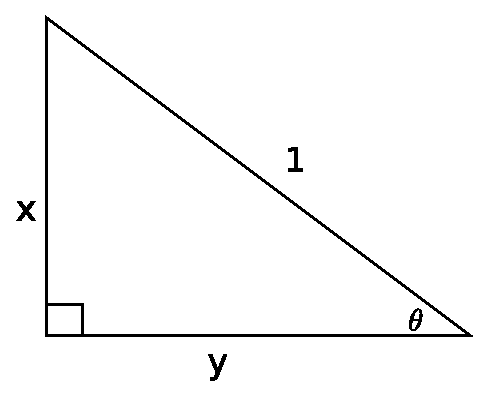
\includegraphics[scale=0.5]{chapters/images/triangle.eps}
\caption{  }
\end{figure} 
\end{itemize}
The remaining expressions are obtained in exactly the same way, and we won't do them here. 



